%!TEX root = these.tex

%\chapterstar{INTRODUCTION}
% Pour des renseignements sur \chapterstar : voir le fichier macros.tex

\chapterstar{Introduction} % "*" pour que l'introduction ne s'affiche pas dans la table des matières, sinon elle s'y affichera comme un chapitre d
% \mtcaddchapter
% \addstarredpart{Introduction} % Pour ajouter une partie ("part") fictive dans la table des matières
% \mtcaddpart
% \markboth{Introduction}{Introduction}  %% header manuel car sinon, ils me marquent le header du dernier \chapter{?} (on est dans un \chapter*{?} )
\selectlanguage{francais}

L'introduction nous permettra tout d'abord de poser le contexte et la problématique liés au sujet de la thèse. Dans un deuxième temps, nous exposerons brièvement l'approche générale choisie afin de répondre à cette problématique et enfin nous présenterons un plan général du manuscrit.

\section*{Contexte et problématique}

Il est possible de diviser la biologie structurale et donc l'étude théorique de structures moléculaires en trois activités principales organisées selon le processus séquentiel suivant (également illustré dans la Figure \ref{}): (1) la \textbf{collecte de données} par les expérimentations, (2) la \textbf{modélisation moléculaire} et (3) la \textbf{simulation moléculaire} des structures 3d. Chacune de ces étapes met en jeu des outils de visualisation et d'analyses permettant de contrôler les données générées, les interpréter pour les étapes suivantes et enfin les utiliser comme nouvelles connaissances afin d'établir de nouvelles hypothèses scientifiques. Il n'est pas rare que plusieurs itérations de ce processus soient nécessaires à l'établissement d'une conclusion scientifique significative pour le phénomène biologique étudié. Chaque nouveau processus prenant comme données d'entrée une partie des résultats générés par l'analyse des données du processus précédent.

\begin{figure}[h]
  \centering
  {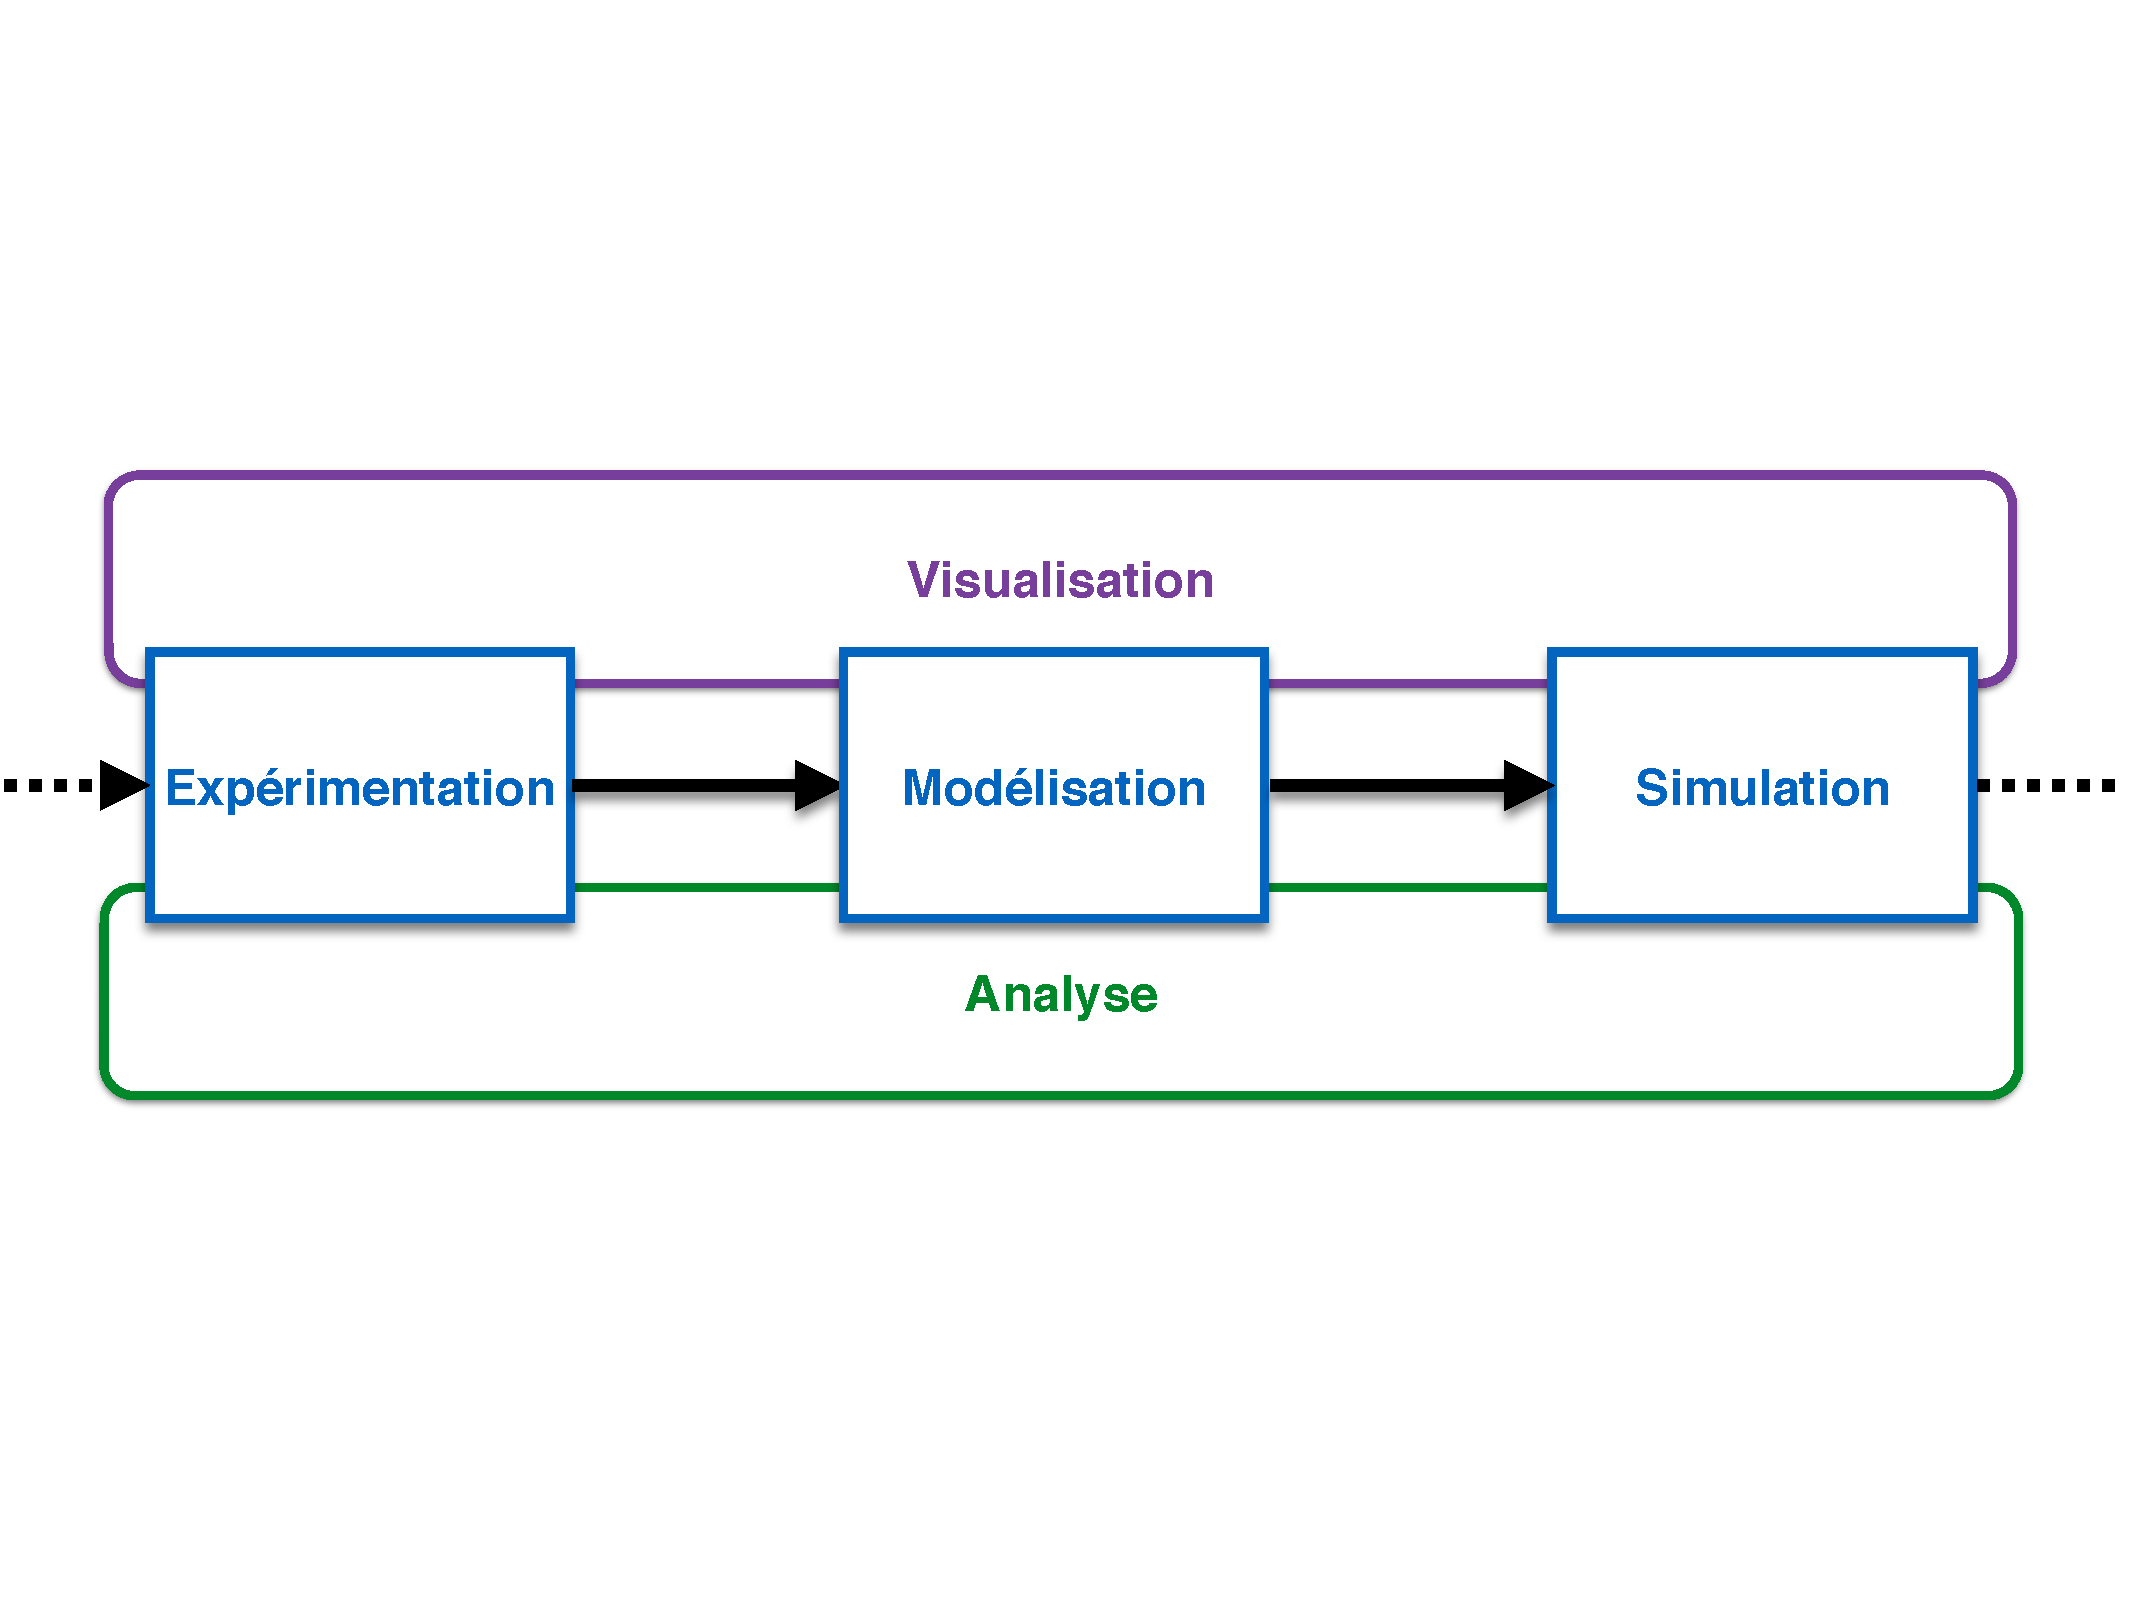
\includegraphics[width=.75\linewidth]{./figures/ch1/process_bio_struct}}
    \caption{{\it Schéma du processus itératif d'étude d'une structure moléculaire en biologie structurale. Les trois grandes étapes sont représentées en bleu, les outils de visualisation et d'analyses présents tout au long du processus sont représentés respectivement en violet et vert.}}
  \label{Fig:VR_pubmed_trend}
  \hspace{0.2cm}
\end{figure}

Au sein de ce processus, la performance croissante des outils de calcul informatique permet aujourd'hui de générer des volumes de données considérables. La biologie structurale voit la \textbf{précision} et la \textbf{taille} de ses modèles moléculaires augmenter rapidement. Cette complexité grandissante est rendue possible par l'efficacité croissante des programmes de simulation numérique moléculaire. Ces derniers peuvent désormais générer des images décrivant l'évolution temporelle de structures moléculaires pouvant atteindre plusieurs \textbf{millions} de particules à une précision \textbf{atomique} \cite{sanbonmatsu2013molecular}. Les méthodes de manipulation fournies par les logiciels de visualisation moléculaire se retrouvent limitées dans leur efficacité pour explorer de tels complexes.
\textbf{Représenter et appréhender ces complexes moléculaire de grande taille est devenu un besoin crucial pour en extraire des informations.} 

Mais l'étape de visualisation n'est pas la seule victime de l'amélioration des moyens de calcul. Cette efficacité croissante n'est malheureusement pas directement corrélée à l'augmentation des moyens d'analyse et la quantité générée de données est bien souvent très supérieure à la quantité de données pouvant être traitée par les experts scientifiques. De même, les capacités de calcul ont depuis longtemps dépassé les capacités de stockage, pourtant elles-mêmes en croissance permanente \cite{zimmerman2014data}. Enfin, la taille des données impacte directement l'efficacité et la rapidité des échanges de données entre les centres de calcul et les laboratoires de biologie. La minimisation des échanges de données, de la quantité de données à stocker et à analyser est donc aujourd'hui un enjeu crucial pour le traitement des données scientifiques.

L'ajout d'un moyen de contrôle sur la génération des données, parallèlement à la simulation, pourrait permettre de filtrer les données obtenues. Ce filtre doit cependant être impérativement \textbf{sans conséquences} pour la compréhension finale du phénomène étudié. L'approche \textit{in situ} répond en partie à cette problématique en mettant en place une solution permettant le calcul, l'analyse et le rendu de données grâce à des solutions technologiques de haute performance autorisant le suivi en temps interactif d'une simulation moléculaire \cite{dreher_interactive_2013,kuhlen2011parallel,ma2009situ}. L'utilisateur a donc la possibilité d'influer sur sa simulation en fonction des données qu'il visualise.

Cependant, la simulation étant souvent déportée sur des sites de calcul distants, se pose la question de la sécurité des données qui transitent entre des sites distants et la difficulté pour y accéder afin de mettre en place une interface efficace. L'approche \textit{in situ} souffre d'une limitation importante de ses performances lorsque elle est utilisée en dehors d'infrastructures dédiées aux communications entre les centres de calcul et les laboratoires, la quantité de données échangée étant souvent supérieure aux capacités d'échange des réseaux standards. Ces limitations techniques freinent donc les possibilités d'interactions communes entre la simulation, le rendu et les analyses et induisent souvent une \textbf{dissociation} de ces modules. L'utilisateur doit donc manipuler les données hétérogènes provenant de chacune des étapes de sa simulation de façon indépendante et cloisonnée. Son contrôle et le filtre qu'il pourra effectuer sur les données mises en jeu devra passer par une planification des tâches en amont de la simulation.

Le positionnement de l'expert scientifique au centre de la boucle de décision et de ce fait au centre du processus d'étude d'une structure passe donc par la mise en place d'éléments d'analyse et de visualisation liés de façon à ce que l'utilisateur puisse appréhender le phénomène observé dans son ensemble pour intervenir à tout instant du processus de simulation. 
L'articulation entre visualisation et analyse est donc primordiale et doit passer par un espace de travail commun et mixte qui rassemblera ces deux étapes du processus de biologie structurale. \textbf{Il s’agit concrètement de présenter de manière conjointe et simultanée les structures moléculaires et leurs analyses et de permettre leur manipulation par des interactions directes.}

La biologie structurale a toujours su intégrer au sein de chacune de ses étapes l'outil informatique. Du traitement des signaux des méthodes expérimentales jusqu'à la visualisation de structures 3d, les avancées technologiques ont toujours trouvé un écho au coeur de ses outils.
Parmi ces nouvelles technologies, la Réalité Virtuelle constitue une progression majeure dans l'appréhension des contenus virtuels 3d et s'impose aujourd'hui comme l'un des domaines les plus actifs et les plus attractifs pour les investissements des grandes entreprises du secteur de la haute technologie.
Elle est associée à des espaces d'affichage étendu par le biais de dispositifs de grande taille où l'utilisateur peut évoluer tout en conservant un point de vue adapté et cohérent à sa position et son orientation par rapport à l'objet observé (systèmes CAVE, murs d'écrans, etc...), ou par des dispositifs de taille plus réduite et portable mais à travers lesquels l'utilisateur peut également percevoir un monde virtuel à 360 degrés grâce à un suivi de l'orientation de sa tête (casques stéréoscopiques, etc...). Les canaux auditifs et tactiles sont également au centre des considérations de la RV. L'audio 3d permettant de simuler des sources audio dans un environnement 3d autour de l'utilisateur et les retours haptiques associés à certains dispositifs d'interaction permettent de simuler une dimension tangible lors de l'interaction de l'utilisateur avec l'environnement virtuel. Ces canaux constituent tout deux des approches supplémentaires pour immerger davantage l'utilisateur au sein de données virtuelles qu'il étudie.

De la même manière que les moeurs tendent à évoluer vers des supports immersifs, la biologie structurale sera certainement amener à suivre ce bousculement des usages. 
La RV offre en effet une perception stéréoscopique de haute qualité, atout certain pour une meilleure compréhension des données moléculaires intrinsèquement tridimensionnelles \cite{van2000immersive,stone_immersive_2010,odonoghue_visualization_2010}. Elle est également pourvoyeuse de contextes interactifs favorisant la manipulation directes de données virtuelles. Elle se caractérise par des interactions plus naturelles déclenchées par des interactions directes avec les objets virtuels présentés via des gestes et/ou par des commandes vocales \cite{bowman2001design}.

Cependant, l'immersion comporte quelques limites et étapes à franchir avant de pouvoir constituer un outil totalement fonctionnel pour la biologie structurale. 
La navigation au sein de dispositifs immersifs dans des données abstraites est un \textbf{premier obstacle}. Découlant de la navigation au sein de scènes virtuelles immersives et également présent pour des scènes réalistes, par opposition aux scènes illustrant des données abstraites, le mal du simulateur est un frein non négligeable à l'expérience de l'utilisateur. Ce phénomène de gène pour l'utilisateur dégrade significativement son expérience et ses performances dans les environnements immersifs. Plusieurs études ont montré que ce mal du simulateur possède plusieurs points communs avec le mal des transports \cite{laviola_jr_discussion_2000}. De la même façon que pour le mal des transports, dans un environnement immersif, le cerveau éprouve une certaine difficulté à dissocier les retours visuels de la scène virtuelle aux sollicitation physiques incohérentes ou inexistantes prenant place au même instant. Cette dissociation de la sollicitation du système vestibulaire par rapport au système perceptif \cite{reason1975motion} entraîne chez certaines personnes un malaise qui peut aller de légères sensations d'inconfort à de plus importants troubles de l'équilibre ou de nausées. Les paradigmes de navigation en condition immersive sont multiples mais ont souvent été développé pour répondre à des contraintes de navigation dans des scènes réalistes et ne parviennent donc pas à répondre aux attentes d'efficacité requises au sein de scènes virtuelles dont les informations proposées sont de nature différente \cite{trellet_content-guided_2014}. Cette absence de compatibilité entre les scènes réalistes et abstraites peut s'expliquer par: 1) une absence de repères spatiaux dans les scènes abstraites où les données scientifiques ne sont généralement pas exposées au sein d'un environnement mais dans un espace vide monochromatique, 2) une absence de notion d'orientation, sans haut ni bas, 3) une exploration centrée sur un objet unique au centre de l'attention. 
\textbf{Des paradigmes de navigation sont donc un pré-requis majeur pour la mise en place d'un espace de visualisation et d'exploration moléculaire immersif.}

L'intégration des analyses à la visualisation, dans l'optique de fournir un contrôle sur l'ensemble des paramètres et donnés de sa simulation à l'utilisateur constitue un \textit{deuxième obstacle} à franchir pour l'implémentation de la biologie structurale au sein d'environnements immersifs.
Les dispositifs adaptés aux espaces immersifs existent mais ils ne peuvent répondre efficacement au large spectre de tâches propres à la biologie structurale. Parmi ces tâches, la sélection, le changement de rendu graphique, le mouvement et l'accès aux informations sont plusieurs actions indispensables en visualisation moléculaire. A ces commandes s'ajoutent toutes les actions propres aux espaces d'analyse et permettant d'interagir avec des graphes de valeur. 
\textbf{Afin d'optimiser la couche d'interaction entre l'utilisateur et les espaces de travail, il est donc nécessaire de mettre en place une méthode robuste permettant à la fois d'anticiper et de simplifier les étapes d'interaction pour l'exécution de chaque tâche.}


% En parallèle de la navigation, les interactions entre l'utilisateur et son espace de travail dans un environnement immersif sont limitées par l'impossibilité d'utiliser les dispositifs précis des stations de travail fixes. L'obscurité liée aux dispositifs immersifs, couplée à la position debout rendent désuet la paire clavier/souris. La recherche d'une immersion complète de l'utilisateur empêche également la présence de menus et commandes textuelles. Elles sont mis de côté au profit d'interactions plus naturelles déclenchées par des interactions directes avec les objets virtuels présentés via des gestes et/ou par des commandes vocales \cite{bowman2001design}. Plusieurs dispositifs adaptés aux espaces immersifs existent mais ils ne peuvent répondre efficacement au large spectre de tâches propres à la biologie structurale. Parmi ces tâches, la sélection, le changement de rendu graphique, le mouvement et l'accès aux informations sont plusieurs actions indispensables en visualisation moléculaire. A ces commandes s'ajoutent toutes les actions propres aux espaces d'analyse et permettant d'interagir avec des graphes de valeur. 
% Afin de garantir une optimisation de la couche d'interaction entre l'utilisateur et les espaces de travail, il est donc nécessaire de mettre en place une méthode robuste permettant d'anticiper et de simplifier les étapes d'interaction permettant d'accomplir chaque tâche. 

% Afin de répondre aux différentes problématiques exposées précédemment, il fut nécessaire de prendre en compte deux contraintes supplémentaires. Ces contraintes, en filigrane tout au long de notre étude, ont motivé nos choix techniques pour assurer à l'utilisateur une expérience immersive de travail aussi efficace que dans des conditions standards de bureau.
% La première contrainte est la contrainte de temps réel que nous imposent la plupart des environnements immersifs lorsqu'il est question de rendu stéréoscopique s'adaptant au point de vue utilisateur. La réduction de la latence entre les mouvements de l'utilisateur et le rendu calculé pour la nouvelle position et orientation de l'utilisateur à chaque instant fut une  . Nous nous appuyons essentiellement sur des briques techniques et technologiques qui ont déjà prouvé leur efficacité pour le rendu 3d temps réel, il est donc nécessaire que nos apports, en particulier pour la navigation et l'exploration, ne soient pas un frein à l'immersion et au rendu temps réel qui lui est propre.
% La deuxième contrainte temporelle vient de la contrainte interactive inhérente à tout système où l'action de l'utilisateur induit un changement visuel ou structurel de la scène et des informations qu'il perçoit. Cette contrainte en temps interactif fut un point important du développement de notre liaison bi-latérale entre espace d'exploration et espace d'analyses. Ce temps interactif doit se rapprocher au maximum de ce que pourrait attendre l'utilisateur, en terme de retours sensoriels, lors du déclenchement d'une action. Il n'est souvent pas nécessaire que l'action voit sa réalisation s'effectuer en temps réel, c'est pourquoi nous parlerons de temps interactif.

 
\section*{Approche générale}

Motivés par le manque de paradigmes de navigation spécifiques pour domaine de la biologie structural, notre premier axe de travail s'est concentré sur le développement de méthodes de navigation basées sur \textbf{le contenu et la tâche} en biologie structurale. Ces méthodes et paradigmes s'inspirent de la particularité géométrique commune que partagent la plupart des complexes moléculaires : un agencement des sous-unités de façon symétrique \cite{goodsell_structural_2000}. Notre approche n'est néanmoins aucunement contrainte à des complexes moléculaires symétriques puisque toute structure particulière retrouvée au sein d'une molécule nous permet de mettre en place nos paradigmes de navigation. Grâce à ces paradigmes, tout au long de son exploration, l'utilisateur 1) garde un point de vue stable sur son complexe, 2) possède des repères spatiaux fixes afin de se situer dans la scène, 3) peut utiliser des chemins optimaux de déplacement pour atteindre des régions d’intérêt. Ces apports répondent respectivement aux problèmes de malaise pouvant être ressentis à cause: 1) d'une variation trop rapide de l'orientation de l'utilisateur par rapport à sa cible visuelle, 2) d'une perte de la situation spatiale de l'utilisateur dans sa scène, 3) d'un trop grand nombre d'étapes ou de temps pour atteindre une région d'intérêt tout en gardant une conscience spatiale de la scène virtuelle. En contraignant la navigation à des chemins jugés optimaux pour son expérience d'exploration, via une restriction des directions du mouvement et des orientations de la caméra, nous fournissons un carcan de possibilités de navigation limité mais adapté aux interactions pouvant prendre place au sein des environnements immersifs. De la même manière, nous anticipons certaines tâches d'exploration en fournissant des paradigmes automatisant certains déplacements considérés comme habituels en exploration moléculaire.

%%%%%%%%%%%%%%%%%%%%%%%%%%%%%%%%%%%%%%%%%%%%%%%%%%%%%%%%%%%%%%%%%%%%%%%%%%%%

Profitant des techniques de visualisation avancées mises à disposition par la RV, notre seconde démarche fut de fournir un moyen de visualiser simplement mais de façon \textbf{immersive et 3d}, des scènes moléculaires à partir de leur simple rendu graphique \textit{2d}. Cet enrichissement du processus de représentation moléculaire a pu tout d'abord profité de la démocratisation des périphériques mobiles comme support d'utilisation, et ensuite répondre à plusieurs tâches spécifiques de biologie structurale.

La première application de notre outil fut le contrôle de l'évolution d'une simulation moléculaire par un expert scientifique. Ce contrôle doit permettre d'appréhender la direction vers laquelle tend une simulation et mettre ainsi en évidence d'éventuelles évolutions ne respectant pas les contraintes imposées ou présentant des incohérences scientifiques notables. 

Nous proposons un support mobile permettant de visualiser de façon simple et rapide l'état d'une simulation à travers une ou plusieurs photographies de la structure simulée. La légèreté des images utilisées pour ce rendu et le développement axé multi-plateforme de notre application, permet également son utilisation au sein de communications scientifiques diverses (journaux papier, journaux électroniques, actes de conférences, etc...) afin d’accroître la quantité d'information présentée. A la différence des images 2d habituelles, notre méthode permet un rendu pseudo-3d pour des illustrations complexes constituées de plusieurs couches et/ou affichant un objet désirant être affiché en profondeur. 
L'importation d'objets 3d et leur exploration à la manière d'un visualiseur 3d sont également associées à l'application et permettent la manipulation de structures complètes de molécules. Deux méthodes permettent d'appréhender la structure du modèle 3d importé, le premier est basé sur une manipulation simple grâce à un ensemble de rotations et translations, le second propose lui d'utiliser le périphérique mobile à la manière d'une fenêtre sur un monde virtuel entourant l'utilisateur et qu'il peut regarder au travers de son périphérique.

%%%%%%%%%%%%%%%%%%%%%%%%%%%%%%%%%%%%%%%%%%%%%%%%%%%%%%%%%%%%%%%%%%%%%%%%%%%%%

Notre troisième sujet d'études s'intéresse à la possibilité de regrouper les espaces de visualisation et d'analyse afin de raccourcir la boucle d'étude des données de simulation moléculaire et ainsi répondre aux problèmes de surcharge de données. Comme exposé précédemment, dans une situation en temps réel, un enjeu majeur est de réduire les données échangées entre les composants de simulation, de visualisation et d'analyse pour permettre à un utilisateur de contrôler ces trois composants de façon optimale et en temps interactif.

Inspirés par les techniques de visualisation analytique visant à intégrer une certaine interactivité entre les solutions de visualisation et d'analyses \cite{kielman2009foundations}, nous avons chercher à lier les données échangées entre ces solutions afin de pouvoir les manipuler dans un espace de travail commun.
Pour ce faire, notre approche s'est basée sur la mise place une couche d'abstraction supplémentaire décrivant les données manipulées usuellement par les experts du domaine. Cette couche d'abstraction a pu être mise en place par la construction d'une description sémantique des concepts mis en jeu lors de la visualisation et l'analyse de structures moléculaires statiques ou au cours d'une simulation. Cette description fut l'objet de la définition d'une ontologie ayant permis de construire une base de données liées, directement inspirée de ce qui peut être fait dans le web sémantique, afin de regrouper et classifier l'ensemble des données mises en jeu lors d'une session de travail spécifique et regroupant l'ensemble des informations que possède l'expert scientifique sur son système moléculaire \cite{berners2001semantic}. Les utilisateurs possèdent , à travers l'ontologie mise en place, une suite de règles et de descriptions des concepts qu'ils vont manipuler, leur permettant à la fois de comprendre aisément l'organisation de leurs informations scientifiques au sein de l'application mais également d'enrichir cette organisation via l'élargissement de l'ontologie. L'ontologie mise en place permet enfin de garder une homogénéité forte pour chaque nouvelle étude. En définissant les concepts pouvant être utilisés, elle impose en effet un formatage clair des données qui permet finalement un recoupage très aisé des données générées au sein de chaque base de données (dans le cas d'une base de données par cas d'étude) et assure ainsi leur inter-compatibilité.


\section*{Plan du manuscrit}

Nous aborderons l'ensemble de nos contributions et les contextes dans lesquels ils s'inscrivent au travers de 5 chapitres distincts. 
Le \textbf{premier chapitre} fera office de rappel des caractéristiques de la biologie structurale à travers sa définition, ses usages et ses enjeux. Nous identifierons tout d'abord les acteurs et processus du domaine plus large que constitue la biologie moléculaire, nous concentrant principalement sur le coeur de la transformation de l'information génétique en entités effectrices du fonctionnement d'une cellule vivante. Cela nous amènera à cerner la place de la biologie structurale au sein de la biologie moléculaire. Les différentes méthodes et outils caractérisant la biologie structurale seront ensuite énumérées pour finalement énoncer ses limites et recenser ses nouveaux usages.

Le \textbf{second chapitre} mettra en avant l'un des domaines moteurs illustrant ces nouveaux usages, la Réalité Virtuelle. Nous définirons tout d'abord ce domaine à travers trois de ses principaux axes: l'immersion, l'interaction et la navigation. Ses apports à la biologie structurale sont ensuite discutés pour finalement identifier les limites actuelles de son application en biologie structurale.

Nous développerons dans le \textbf{troisième chapitre} nos contributions pour amener la dimension immersive au coeur de trois aspects importants de la biologie structurale: la diffusion au sein de la communauté de structures 3d, le contrôle rapide de l'état d'une simulation numérique moléculaire et l'exploration de complexes moléculaires.

Le \textbf{quatrième chapitre} sera consacré à la présentation d'un domaine pouvant apporter des réponses concrètes à certaines limites de la RV en biologie structurale, la visualisation analytique. A travers plusieurs de ses méthodes et techniques qui seront détaillées, nous mettrons en avant l'apport de la notion d'interactivité qu'elle introduit pour les tâches d'analyses et de visualisation moléculaire. Nous introduirons plus particulièrement comment l'interactivité entre ces deux tâches hétérogènes peut passer par la définition d'un cadre sémantique global. Nous verrons comment ce cadre sémantique peut s'inscrire dans un processus plus large de gestion des données, suivant l'exemple du web sémantique.

Finalement, le \textbf{cinquième chapitre} sera l'implémentation concrète d'une plateforme unique mixant les espaces d'analyses et de visualisation au sein d'un même processus interactif et immersif pour l'utilisateur. Nous montrerons comment les outils du web sémantique peuvent intégrer les données provenant d'études de structures moléculaires. Cette intégration et la plateforme finale seront finalement illustrées et évaluées dans une dernière partie.